% Geometry, font
\documentclass[12pt, letter]{article}
\usepackage[margin=0.8in]{geometry}
\usepackage[T1]{fontenc}
\usepackage{fourier}
\usepackage{titling}
\setlength{\droptitle}{-5em} 
\usepackage[parfill]{parskip}
\usepackage{graphicx}
\graphicspath{{imgs/}}
\usepackage{hyperref}

% Math stuff
\usepackage{amssymb}
\usepackage{bm}
\usepackage{amsmath}

% Code Highlighting
\usepackage{minted}
\usemintedstyle{solarizedlight}

\author{Zach Neveu}
\title{ Day 14 Notes }

\begin{document}
\maketitle

\section{Agenda}%
\label{sec:agenda}
\begin{itemize}
	\item Branch and Bound to solve ILP
	\item Announcements
	\begin{itemize}
		\item Reading
		\item Project due Monday
		\item Quiz Tuesday
	\end{itemize}
\end{itemize}

\section{Branch \& Bound}%
\label{sec:branch_&_bound}
\begin{itemize}
	\item Review of last class example
	\item LP soln is \textbf{optimistic bound} on ILP soln
	\item Add constraints to break up problem into subproblems
	\item Solve each subproblem with LP solver
	\item Repeat recursively until subproblem has integral soln in LP
	\item Don't expand subproblem if\ldots
	\begin{itemize}
		\item Subproblem is infeasible (No LP solns)
		\item LP soln in integral
	\end{itemize}
	\item How to explore graph?
	\item Best soln is to use DFS
	\item Z score of LP soln at parent node is upper bound on Z score of children
	\item This means that branches with low Z scores can be pruned!
	\item Suddenly problem not exponential time any more!
\end{itemize}
\begin{figure}[h]
	\centering
	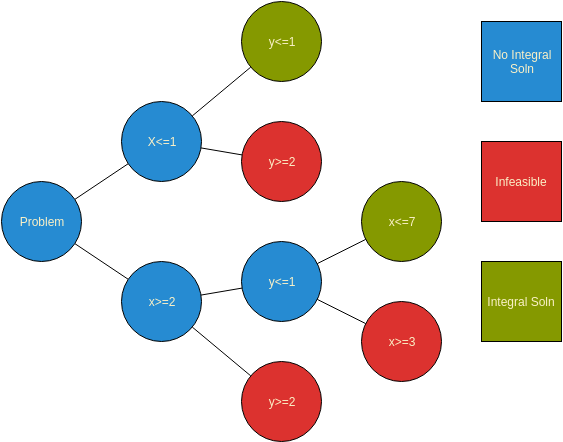
\includegraphics[width=0.8\textwidth]{search}
	\caption{Subproblem Search Diagram}
	\label{fig:search}
\end{figure}

\subsection*{Fathoming Rules: don't expand a subproblem if\ldots}
\begin{enumerate}
	\item Subproblem is infeasible
	\item LP solution is integral
	\item Optimistic bound is worse than the best integral solution found so far
\end{enumerate}

\begin{itemize}
	\item This only prunes if the bound is tight.
	\item Branches with loose bound will not be pruned until far down the tree
	\item LP bound is quite tight
	\item What order to branch variables? $x$ first? $y$ first?
	\item Crucial decision, but no fixed best algorithm - solvers offer choice
	\item \textbf{IDEA:} Try different sized problems with different strategies, find optimal domain for each strategy. Potentially weed out strategies that don't have a region where they are optimal. 
\end{itemize}

\subsection*{Problem Example}
\begin{gather*}
Z = 9x_1+5x_2+6x_3+4x_4 \\
6x_1+3x_3+5x_3+2x_4 \le  10 \\
x_3+x_4 \le 1 \\
-x_1+x_3 \le 0 \\
-x_3+x_4 \le 0 \\
x_i \in \{0, 1\} \\
\end{gather*}

\begin{figure}[h]
	\centering
	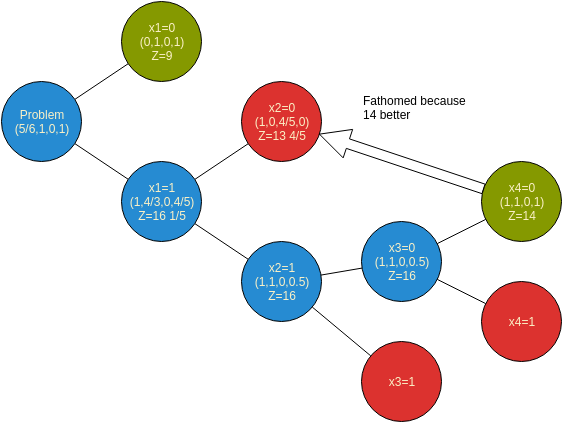
\includegraphics[width=0.8\textwidth]{ex1}
	\caption{Example Problem Search}
	\label{fig:ex1}
\end{figure}

\section{Project Help}%
\label{sec:project_help}

\subsection*{Graph Coloring ILP}
\begin{itemize}
	\item Goal: Minimize Conflicts
	\item Constraints: \# colors, edges
	\item Graph given as list of edges -> constant set param in ampl
	\item Convert into adjacency matrix -> Boolean matrix (numNodes x numNodes)
	\item Possible variables: 
    \begin{itemize}
        \item \texttt{Colors[numNodes] = \{0..numColors\}} -> hard to create linear objective
        \item \texttt{Colors[numNodes,numColors] = \{0,1\}} -> Conflicts easy! Just sum of columns!
    \end{itemize}
\end{itemize}

\begin{table}[h]
    \centering
    \caption{caption}
    \label{tab:label}
    \begin{tabular}{|c|c|c|c|c|}
    \hline
    & c1 & c2 & c3 & c4 \\
    \hline
    node 1 & 0 & 1 & 0 & 0 \\
    \hline
    node 2 & 0 & 1 & 0 & 0 \\
    \hline
    node 3 & 0 & 0 & 1 & 0 \\
    \hline
    conflicts & 0 & 1 & 0 & 0 \\
    \hline
    \end{tabular}
\end{table}

\begin{minted}{Ampl}
param edge {i in 0..numNodes-1, j in 0..numNodes-1} :=
    (if(i,j) in edgelist or (j,i) in edgelist then 1 else 0);
\end{minted}

\section{Advanced ILP Techniques}%
\label{sec:advanced_ilp_techniques}
\subsection*{Fix Variables}
\begin{itemize}
    \item Consider constraint $3x_1\le 2$. $x_1$ must be 0.
    \item $3x_1+x_2 \le 2$: $x_1$ must be 0.
    \item $5x_1+x_2-2x_3 \le 2$: $x_1$ must be 0.
    \item In general, constants bigger than constraint must be set to 0.
\end{itemize}

\subsection*{Eliminate Redundant Constraints}
\begin{itemize}
    \item If constraint depends entirely upon value of different constraint, eliminate it.
\end{itemize}

\begin{gather*}
3x_3-x_5+x_7 \le 1 \\
x_2+x_4+x_0 \le 1 \\
x_1-2x_5+2x_6 \ge 2 \\
x_1+x_2-x_4 \le 0 \\
\end{gather*}

\begin{itemize}
    \item Fix variables
    \begin{itemize}
        \item $x_3 = 0$ 
        \item $x_6 = 1$
        \item $x_5 = 0$ 
        \item $x_2 = 0$
        \item $x_1 = 0$ 
        \item $x_7$ is only real free variable!
    \end{itemize}
\end{itemize}

\subsection*{Cutting Planes}
\begin{itemize}
    \item Consider problem in fig. \ref{fig:cutplane}
    \item Top right corner points are not integral solutions
    \item Can eliminate these infeasible points before sending to solver
    \item Do this elimination by adding a redundant constraint that all integral feasible solutions satisfy
    \item Consider $6x_1+3x_2+5x_3+2x_4 \le 10$ 
    \item If $x_1, x_2, x_4 = 1$, then this doesn't work
    \item Add $x_1+x_2+x_4 \le 2$ to speed up ILP solver.
    \item Without redundant constraint, solver produces $(\frac{5}{6}, 1, 0, 1)$, but the redundant constraint does not allow for this, allowing faster fathoming.
\end{itemize}

\begin{figure}[h]
    \centering
    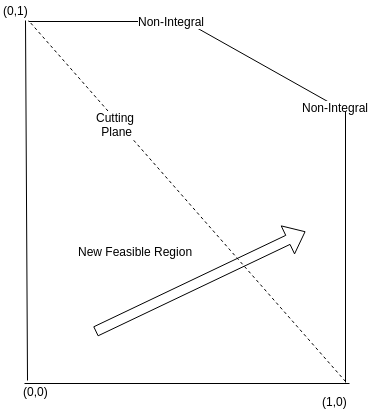
\includegraphics[width=0.4\textwidth]{cutplane}
    \caption{Cutting Plane Example}
    \label{fig:cutplane}
\end{figure}

\end{document}
